\chapter{Módulo: Roles y Permisos}
\label{mod:12-roles-y-permisos}

\section{Propósito}
\label{sec:roles-proposito}

ABM del catálogo de \code{Role}/\code{Permission} y su asignación: define qué combinaciones de permisos existen como ``rol'' seleccionable y qué permisos tiene cada uno. Es el panel de configuración detrás de la autorización descrita en el Capítulo~\ref{mod:01-identidad-y-acceso} --- aquí se define \emph{qué puede hacer cada rol}, allí se gestiona \emph{qué rol tiene cada usuario}.

\section{Entidades principales}
\label{sec:roles-entidades}

Ver Capítulo~\ref{sec:modelo-datos}, Grupo A.

\begin{longtable}{p{3.0cm}p{10.3cm}}
\caption{Entidades principales del módulo de Roles y Permisos.}\label{tab:roles-entidades}\\
\toprule
\textbf{Entidad} & \textbf{Rol} \\
\midrule
\endfirsthead
\toprule
\textbf{Entidad} & \textbf{Rol} \\
\midrule
\endhead
\bottomrule
\endfoot
\code{Role} & Rol configurable con nombre. \code{Type} (\code{admin}$\vert$\code{professional}$\vert$\code{patient}, nullable e \textbf{inmutable}) marca los 3 roles de sistema. \\
\code{Permission} & Catálogo fijo de 56 permisos granulares sembrados por \code{DbSeeder.}\allowbreak \code{AllPermissions} (\code{ver_pacientes}, \code{crear_venta}, \code{gestionar_}\allowbreak \code{laboratorio}, etc.). 55 tienen policy homónima en \code{Program.cs}; la excepción es \code{ver_recepcion}, que está en el seed pero \textbf{no} tiene policy declarada --- no se puede usar hoy en un \code{[Authorize(Policy=.}\allowbreak \code{.}\allowbreak \code{.}\allowbreak \code{)]} aunque exista en la base. \\
\code{RolePermission} & Pivote many-to-many --- la asignación real de permisos a un rol. \\
\end{longtable}

\section{Reglas de negocio clave}
\label{sec:roles-reglas}

\begin{itemize}
  \item \textbf{Un \code{Role} es solo un nombre más una colección de \code{Permission}s} --- no hay lógica de negocio codificada por nombre de rol en ningún endpoint. Ver \hyperref[adr:0003]{ADR 0003}.
  \item \textbf{Se pueden crear roles ad-hoc desde \code{/roles} sin modificar código ni desplegar} --- ej.\ ``Recepcionista Senior'' con un permiso extra sobre ``Recepcionista'' --- porque la autorización nunca consulta \code{Role.Name}, solo los permisos resueltos en el JWT.
  \item \textbf{\code{Role.Type} es inmutable y no es un permiso} --- identifica los 3 roles de sistema (\code{admin}, \code{professional}, \code{patient}) para lógica interna puntual (ej.\ bootstrap del usuario admin, o que el seeder sepa a qué rol darle todos los permisos). No participa en ninguna policy de autorización de endpoint.
  \item \textbf{El admin tiene todos los permisos excepto \code{ver_mis_turnos}} (ese es específico del portal de autogestión del paciente) --- sembrado por el \code{DbSeeder}, no codificado de forma fija en cada policy.
  \item \textbf{Vista propia separada de la gestión de usuarios:} \code{RolesView}/\code{RolFormView} (cards por módulo de negocio, para elegir permisos agrupados visualmente) es una pantalla distinta de \code{UsuariosView} --- esta última solo asigna \emph{qué rol} tiene cada usuario, no edita el contenido de un rol. Decisión de diseño explícita para no mezclar ambas responsabilidades en una sola pantalla.
\end{itemize}

\section{Endpoints}
\label{sec:roles-endpoints}

Detalle completo en el Apéndice de Referencia de API, \S 1 (\code{RolesController}, \code{User}\allowbreak \code{Roles}\allowbreak \code{Controller} --- ambos viven en el mismo archivo \code{RolesController.}\allowbreak \code{cs}).

\begin{longtable}{p{3.5cm}p{4.6cm}p{5.9cm}}
\caption{Endpoints principales del módulo de Roles y Permisos.}\label{tab:roles-endpoints}\\
\toprule
\textbf{Método} & \textbf{Ruta} & \textbf{Descripción} \\
\midrule
\endfirsthead
\toprule
\textbf{Método} & \textbf{Ruta} & \textbf{Descripción} \\
\midrule
\endhead
\bottomrule
\endfoot
GET & \code{/api/roles} & Listado de roles \\
GET & \code{/api/roles/{id}} & Detalle (incluye sus permisos) \\
POST/PUT/DELETE & \code{/api/roles} & ABM del rol y su combinación de permisos \\
GET & \code{/api/roles/{id}/users} & Usuarios que tienen ese rol \\
GET/POST/DELETE & \code{/}\allowbreak \code{api/}\allowbreak \code{users/}\allowbreak \code{{userId}/roles} & Asignación de roles a un usuario (documentado también en el Capítulo~\ref{mod:01-identidad-y-acceso}, vive en \code{UsuariosView}) \\
\end{longtable}

\section{Flujo típico}
\label{sec:roles-flujo}

CRUD estándar sin pasos multi-capa no triviales --- no amerita diagrama de secuencia. La única mecánica particular es que el formulario de rol (\code{RolFormView}) presenta los 55 \code{Permission} agrupados por módulo de negocio (cards), y guarda la selección completa como el nuevo set de \code{RolePermission} del rol (reemplazo total, no diffing incremental).

\section{Vistas de frontend}
\label{sec:roles-vistas}

\begin{itemize}
  \item \code{RolesView.vue} (listado)
  \item \code{RolFormView.vue} (alta/edición, cards de permisos por módulo)
\end{itemize}

\section{Interfaz}
\label{sec:roles-interfaz}

\begin{figure}[htbp]
\centering
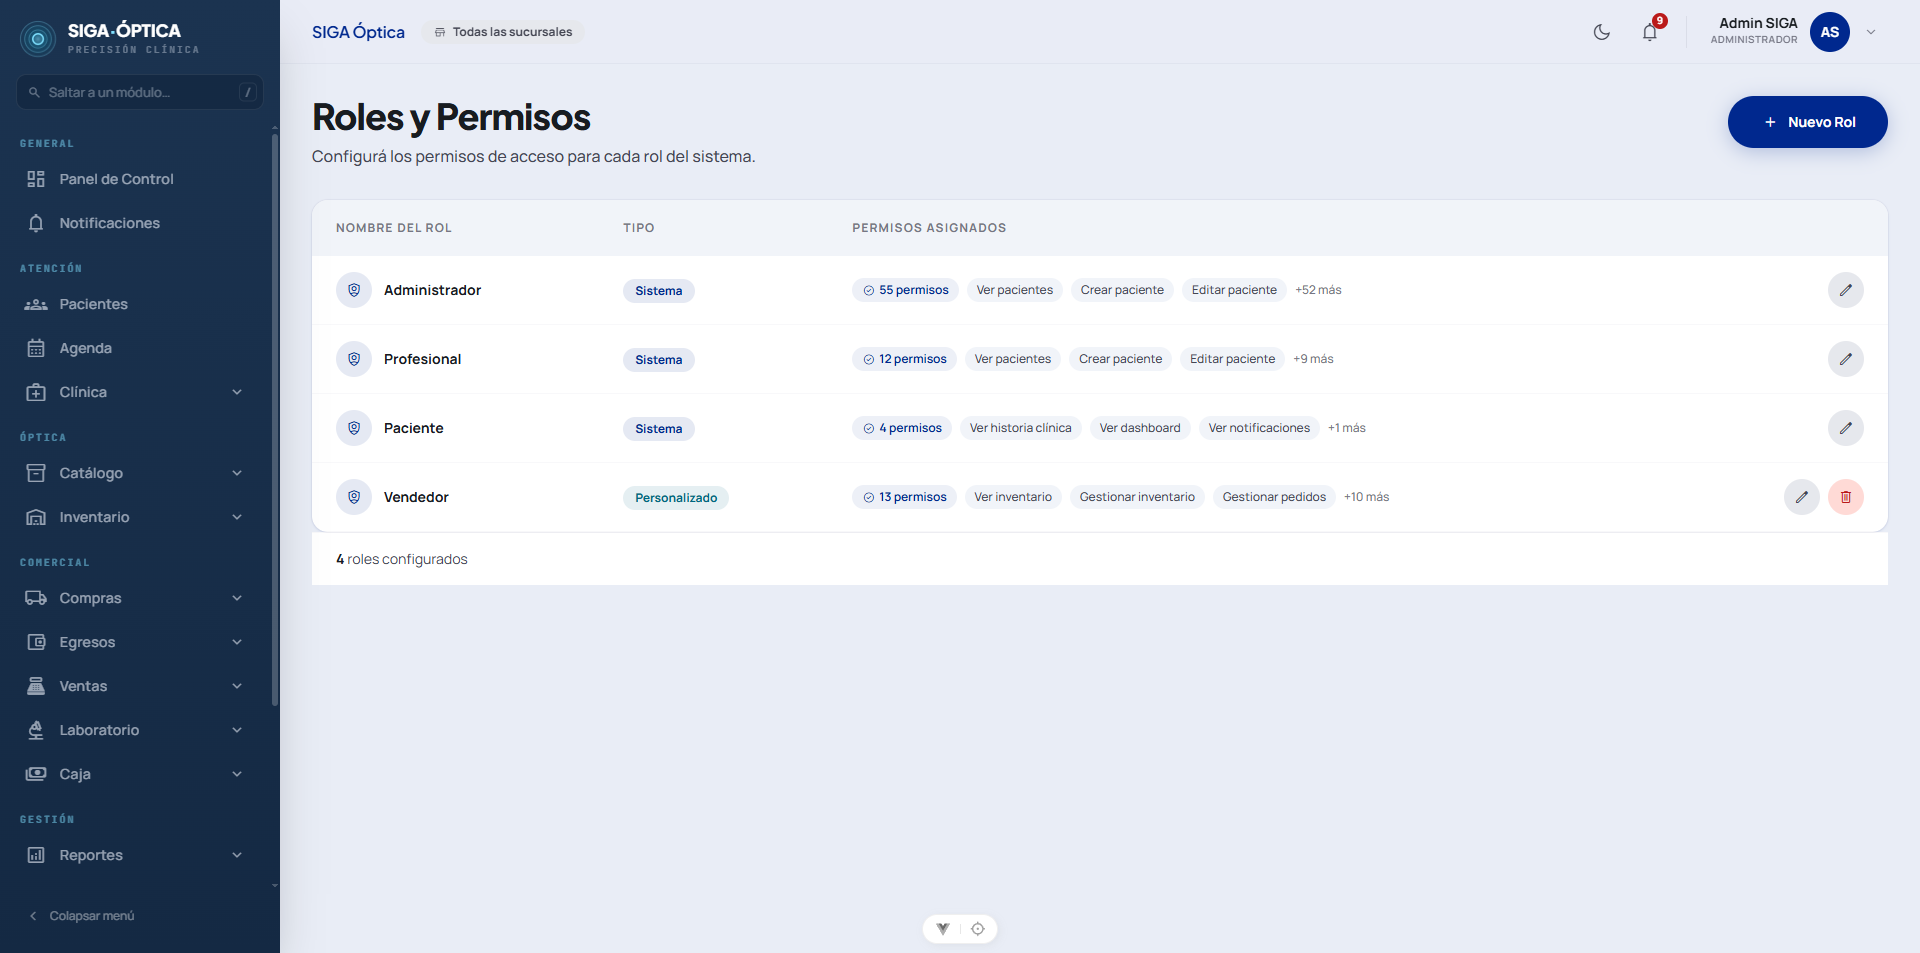
\includegraphics[width=0.95\textwidth]{imagenes/mod12-roles.png}
\caption{Roles del sistema con la cantidad de permisos asignados a cada uno.}
\label{fig:mod12-roles}
\end{figure}

\section{Estado}
\label{sec:roles-estado}

\Implementado.
